

%%% This LaTeX source document can be used as the basis for your technical
%%% report. Intentionally stripped and simplified
%%% and commands should be adjusted for your particular paper - title, 
%%% author, citations, equations, etc.
% % Citations/references are in report.bib 

\documentclass[conference,backref=page]{acmsiggraph}
\usepackage{algorithm2e}
\usepackage{graphicx}
\usepackage{pgfplots}
\TOGonlineid{45678}
\TOGvolume{0}
\TOGnumber{0}
\TOGarticleDOI{1111111.2222222}
\TOGprojectURL{}
\TOGvideoURL{}
\TOGdataURL{}
\TOGcodeURL{}

% Include this so that citations show up in blue and the page information is included in the reference section
\hypersetup{
    colorlinks = true, 
    linkcolor = blue,
    anchorcolor = red,
    citecolor = blue, 
    filecolor = red, 
}
\title{Travelling Salesman Problem\\
	   Report}

\author{Conner Weatherston \thanks{e-mail:40167111@live.napier.ac.uk} \\
Edinburgh Napier University\\
Algorithms and Data Structures (SET09117)}
\pdfauthor{Conner Weatherston}

\keywords{travelling salesman problem, nearest neighbour, optimisation, algorithms, big o}

\begin{document}

\maketitle

\raggedbottom

\begin{abstract}

The purpose of this report is to find out the efficiency of the nearest neighbour algorithm in order to solve a  variety of travelling salesman problems. This report is also looking how possible variations and optimization techniques such as just searching on an individual axis would impact on the performance of the algorithm. From the results it can be concluded that is quicker to compare on a single axis and to reduce the number of mathematical operations used. Reducing code in the loop also improves the algorithm significantly. Out of the different variations of the nearest neighbour the most practical one to use would be the nearest neighbour squared.
\end{abstract}



\keywordlist


\section{Introduction}

This report is looking at possible improvements of the nearest neighbour algorithm in order to solve the travelling salesman problem (commonly referred to as tsp). The tsp essentially is a question which asks 'Given a set of cities, what is the shortest route possible that visits each city only once and will return to the origin\cite{tsp}.

The main issue with the travelling salesman problem is the possible routes available to traverse grows exponential with size. An example of this is in a tsp with 10 cities there are 181,400 possible routes that can be taken. This number is calculated using the formula:
 \begin{equation}
P =  \frac{(N-1)!}{2}
\end{equation}
where~$P$ is number of possibilities and~$N$ is number of cities (points).


Only half of the possible routes are counted as each route has an equal reverse route that has the exact same distance. The ~$P$-1 is there since the starting city is always defined and the other cities can have different permutations.

\begin{center}
	\begin{tabular}{| l | l | l | l |}
		\hline
		Size& Possible routes\\ \hline
		5 & 12 \\ \hline
		10 & 181400 \\ \hline
		12 & 19958400 \\ \hline
		14 & 3113510400 \\ \hline
	\end{tabular}
\end{center}

As seen from the table above it is clear that the is an exponential growth in the number of possible routes as the number of cities in the list increases. Due to this brute force methods that search through each possible route is not possible in large data sets. Therefore algorithms are needed that provide a decent route in a reasonable period of time. 

\section{Method}

One of the most common ways to get a general solution to the travelling salesman problem is to utilise the nearest neighbour algorithm. The aim of this algorithm is to sort the list so that the next element is the closest one to the current city. The limiting factor of this algorithm is how fast it can do the comparisons between the current city to the other cities to find the closest one.

\begin{figure}[h]
	
\cite{nn} provides a quick pro and con list for the nearest neighbour algorithm.\\
\begin{center}
\underline{Pros}
\end{center}
\begin{itemize}
	\item Easy to implement.
	\item Very quick results for small data sizes.
	\item Simple to calculate the big O notation.
	
\end{itemize}
\begin{center}
\underline{Cons}
\end{center}
\begin{itemize}
	\item Requires large storage of data. 
	\item Large searching problems (Have to continually iterate over list until it is empty.)
	\item Assumptions are made about distance (Some routes may be infeasible).
\end{itemize}
\caption{Pros and cons of nearest neighbour.}
\end{figure}
\paragraph{Pseudocode} \hfill

In this section the pseudo code for all of the different variations of the algorithm that are aimed to be implemented are available. Algorithm \ref{nn} provides the pseudocode for nearest neighbour.

\begin{algorithm}[h]	
	\KwData{ArrayList input}
	\KwResult{returns Nearest Neighbour list}
	current city = input first value\\
	\While{cities in input}{
		add current city to result\\
		distance = max value\\
		\ForEach{city in input}
		{
			\If{distance(current city, city) $<$ distance}{
				closest city = city\\
				distance = distance(current point,city)\\
			}
		}
		remove closest city from input\\
		current city = closest city\\
	}
\caption{Nearest neighbour algorithm}
\label{nn}

\end{algorithm}

An improvement to the nearest neighbour can be made by using the distance squared function instead of the distance function. To improve upon this more the result from distance squared is stored so it is not needed to be computed again. Algorithm \ref{nns} shows how it should look like.

\begin{algorithm}[h]	
	\KwData{ArrayList input}
	\KwResult{returns Nearest Neighbour squared list}
	current city = input first value\\
	\While{cities in input}{
		add current city to result\\
		distance = max value\\
		\ForEach{city in input}
		{
			current Distance = distanceSquared(current city, city) 
			\If{ current Distance $<$ distance}{
				closest city = city\\
				distance = current Distance.\\
			}
		}
		remove closest city from input\\
		current city = closest city\\
	}
\caption{Nearest Neighbour squared}
\label{nns}
\end{algorithm}\hfill

An attempt of rewriting the algorithm was done. The aim of this was to try and minimise the number of iterations in the for loop by comparing the current distance against the next city in the list. See algorithm \ref{nnre}.
\begin{algorithm}[h]
	\KwData{ArrayList input}
	\KwResult{returns Nearest Neighbour rewritten list}
	current city = input first value\\
	\While{cities in input}
	{
		add current city to result\\
		distance = max value\\
		\ForEach{city in input}
		{
			\If{distance(current city, city) $<$ distance}
			{
				closest city = city\\
				distance = distance(current point,city)\\
			}
			\If{(another city after city)}
			{
				\If{distance(current city, next city) $<$ distance}
				{
					
					closest city = next city \\
					distance = distance(current point, nextcity)\\
					continue loop from next city\\
				}
			}
		}
		remove closest city from input\\
		current city = closest city\\
	}
	\caption{Nearest Neighbour Rewritten algorithm}
	\label{nnre}
\end{algorithm}


Java has a random function available. One variation was crossing a random starting position in order to provide a better result. See algorithm \ref{nnrs}.


	\begin{algorithm}[h]	
		\KwData{ArrayList input}
		\KwResult{returns Nearest Neighbour random start list}
		current city = Random value from input list\\
		\While{cities in input}{
			add current city to result\\
			distance = max value\\
			\ForEach{city in input}
			{
				\If{distance(current city, city) $<$ distance}{
					closest city = city\\
					distance = distance(current point,city)\\
				}
			}
			remove closest city from input\\
			current city = closest city\\
		}
		\caption{Nearest neighbour random start algorithm}
		\label{nnrs}
	\end{algorithm}	
Taking advantage of the collections type it is possible to 	randomise the entire input arrayList before using the nearest neighbour algorithm.
		

\begin{algorithm}[h]	
	\KwData{ArrayList input}
	\KwResult{returns Nearest Neighbour shuffle list}
	input = randomise(input)
	current city = input first value\\
	\While{cities in input}{
		add current city to result\\
		distance = max value\\
		\ForEach{city in input}
		{
			\If{distance(current city, city) $<$ distance}{
				closest city = city\\
				distance = distance(current point,city)\\
			}
		}
		remove closest city from input\\
		current city = closest city\\
	}
	\caption{Nearest neighbour shuffle algorithm}
\end{algorithm}

For the algorithms that use random features (random start and shuffle) it is important to note that 1. They are not reliable methods to calculate a suitable route and secondly given enough time the algorithm could be looped and compared to find out if the new results beat the previous results and if it does replace the results with the new results. However as it is unreliable it was decided to be implemented to see how much it would decrease or increase performance and was not focusing on providing the best route possible (which could happen on its first iteration or it could never happen). 


Another variation of the nearest neighbour is checking for the closest point on a given axis. As the points are in two dimensional space this means checking along the x axis and y axis. The aim of this was to try and completely remove mathematical operations and only use simple boolean operations in order to get a route in quick computation time. However this may result in very long routes due to point distributions. Algorithm \ref{nnx} and algorithm \ref{nny} demonstrate what this would look like.

\begin{algorithm}[h]
	\KwData{ArrayList input}
	\KwResult{returns Nearest x Neighbour list}
	current city = input first value\\
	\While{cities in input}{
		add current city to result\\
		closest x = max value\\
		\ForEach{city in input}
		{
			\If{city.x $<$ current city.x}
			{
				closest city = city\\
				closest x = city.x\\
			}
		}
		remove closest city from input\\
		current city = closest city\\
	}
	\caption{Nearest x neighbour algorithm}
	\label{nnx}
\end{algorithm}

\begin{algorithm}[h]
	\KwData{ArrayList input}
	\KwResult{returns Nearest y Neighbour list}
	current city = input first value\\
	\While{cities in input}{
		add current city to result\\
		closest y = max value\\
		\ForEach{city in input}
		{
			\If{city.y $<$ current city.y}
			{
				closest city = city\\
				closest y = city.y\\
			}
		}
		remove closest city from input\\
		current city = closest city\\
	}
	\caption{Nearest y neighbour algorithm}
	\label{nny}
\end{algorithm}

\pagebreak
\paragraph{O notation} \hfill
 
\begin{figure}[h]
	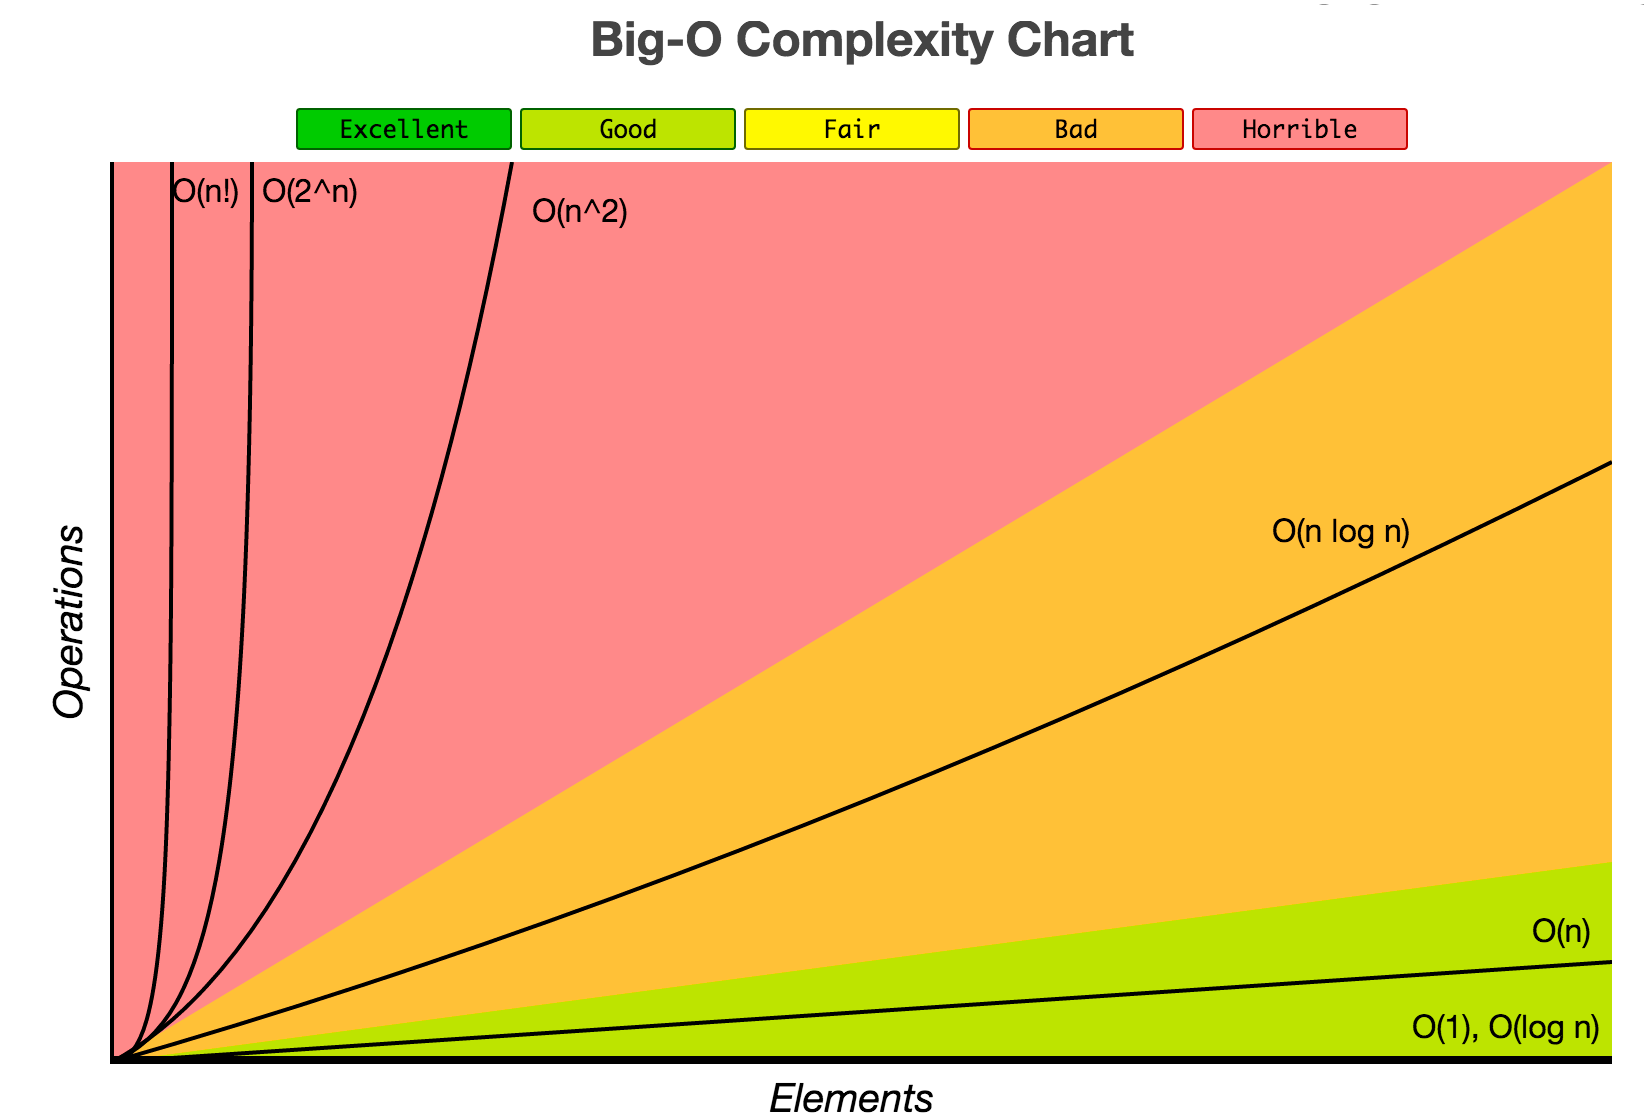
\includegraphics[width=\columnwidth]{images/OCheatSheet.png}
	\caption{Approximate graph for big O complexity.}
	\label{O}
\end{figure}
An effective way to calculate the complexity of an algorithm is to find out what the O notation of the algorithm is. The O notation being used to calculate the complexity is Big O which is used to specifically used to describe the worst-case scenario of an algorithm. 
Figure \ref{O} shows the rough guidelines for big O complexity (From \cite{bigo}). 

To calculate the big O notation of an algorithm a series of rules are followed.
\begin{itemize}
	\item Input will be called n.
	\item Measure the number of "touches" (interactions with n).
	\item It is the worst case scenario.
	
\end{itemize}

The O notation of the nearest neighbour is \begin{math}{n^2} \end{math}. Using the chart for reference it can be judged before results that the complexity is not good. This is because it has a nest for loop (A while loop is a form of the for loop).



It is important to note that complexity has an effect on the performance however performance does not affect the complexity of an algorithm. The reason the specifications of the computer being used is because performance is also affected by hardware.

A limitation of this solution is the file reader. It can only read in certain travelling salesman problems which limits the variety of the results obtained. Another limitation is due to the complexity as the data size increases the time taken to compute will also increase therefore once a certain size is achieved it will take to long to compute in a reasonable time.
\section{Results}

The algorithms were tested using Eclipse Neon.1 Java development environment. Also the machine specifications are as follows:
\begin{itemize}
\item Processor:	Intel i7-4790K @ 4.00GHz
\item Graphics card:	GeForce GTX 980	4GB GDDR5
\item Ram:	16.0G

\end{itemize}

When collecting the results it was important to ensure that they are all treated equally with no bias. Therefore for each data set each algorithm is ran an equal number of times. For this report 5 times was suitable due to the number of data sets and number of variations of the algorithm. The slowest and fastest times were removed and ran again to make the results a little more accurate. This was to take into account of Java garbage collection. Also the algorithms were ran one at a time to ensure there was no heap space competition. Lastly no background applications were running to attempt to minimise any performance issues due to resource competition because of background applications. Another important thing to note is the algorithms were all ran on the same computer to ensure that the hardware specifications remained the same and would not skew the results.
/paragraph{}
The reason for the multiple data sets was to ensure that the solution was valid over a wide range of problems.
\paragraph{Data set Berlin52} \hfill

berlin52 has a size of 52 and when unsorted has a total distance of 22205.61m

\begin{center}	
	
	Nearest Neighbour
	\begin{tabular}{| l | l | l | l |}
		\hline
		& Total Distance(m)& Time Taken (ms)\\ \hline
		Average & 8980.92 & 0.45 \\ \hline
	\end{tabular}
	
	Nearest Neighbour Random Start
	\begin{tabular}{| l | l | l | l |}
		\hline
		& Total Distance (m) & Time Taken (ms)\\ \hline
		Average & 326226.14 & 0.53 \\ \hline
	\end{tabular}
	
	Nearest Neighbour Shuffle
	\begin{tabular}{| l | l | l | l |}
		\hline
		& Total Distance (m) & Time Taken (ms)\\ \hline
		Average & 313703.70 & 0.50 \\ \hline
	\end{tabular}
	
	Nearest Neighbour SQ
	\begin{tabular}{| l | l | l | l |}
		\hline
		& Total Distance (m) & Time Taken (ms)\\ \hline
		Average & 8980.92 & 0.46 \\ \hline
	\end{tabular}
	
	Nearest Neighbour Rewrite
	\begin{tabular}{| l | l | l | l |}
		\hline
		& Total Distance (m) & Time Taken (ms)\\ \hline
		Average & 8980.92 & 0.59 \\ \hline
	\end{tabular}
	
	
	Nearest X Neighbour	
	\begin{tabular}{| l | l | l | l |}
		\hline
		& Total Distance (m) & Time Taken (ms)\\ \hline
		Average & 17074.13 & 0.39 \\ \hline	
	\end{tabular}
	
	Nearest Y Neighbour	
	\begin{tabular}{| l | l | l | l |}
		\hline
		& Total Distance (m) & Time Taken (ms)\\ \hline
		Average & 24438.27 & 0.38 \\ \hline
	\end{tabular}
\end{center}


\paragraph{Data set rl1304} \hfill

rl1304 has a size of 1304 and when unsorted has a total distance of 3231697.34
																				
\begin{center}	
	
	Nearest Neighbour
	\begin{tabular}{| l | l | l | l |}
		\hline
		& Total Distance(m)& Time Taken (ms)\\ \hline
		Average & 339797.47 & 12 \\ \hline
	\end{tabular}
	
	Nearest Neighbour Random Start
	\begin{tabular}{| l | l | l | l |}
		\hline
		& Total Distance (m) & Time Taken (ms)\\ \hline
		Average & 326226.14 & 13 \\ \hline
	\end{tabular}
	
	Nearest Neighbour Shuffle
	\begin{tabular}{| l | l | l | l |}
		\hline
		& Total Distance (m) & Time Taken (ms)\\ \hline
		Average & 313703.70 & 16 \\ \hline
	\end{tabular}
	
	Nearest Neighbour SQ
	\begin{tabular}{| l | l | l | l |}
		\hline
		& Total Distance (m) & Time Taken (ms)\\ \hline
		Average & 339797.47 & 9 \\ \hline
	\end{tabular}
	
	Nearest Neighbour Rewrite
	\begin{tabular}{| l | l | l | l |}
		\hline
		& Total Distance (m) & Time Taken (ms)\\ \hline
		Average & 339797.47 & 23 \\ \hline
	\end{tabular}
	
	
	Nearest X Neighbour	
	\begin{tabular}{| l | l | l | l |}
		\hline
		& Total Distance (m) & Time Taken (ms)\\ \hline
		Average & 3718084.59 & 7 \\ \hline	
	\end{tabular}
	
	Nearest Y Neighbour	
	\begin{tabular}{| l | l | l | l |}
		\hline
		& Total Distance (m) & Time Taken (ms)\\ \hline
		Average & 2786850.75 & 10 \\ \hline
	\end{tabular}
\end{center}

\paragraph{Data set rl1323} \hfill

rl1323 has a size of 1323 and when unsorted has a total distance of 3088180.39. 

\begin{center}	
	
	Nearest Neighbour
	\begin{tabular}{| l | l | l | l |}
		\hline
		& Total Distance(m)& Time Taken (ms)\\ \hline
		Average & 332094.97 & 12 \\ \hline
	\end{tabular}
	
	Nearest Neighbour Random Start
	\begin{tabular}{| l | l | l | l |}
		\hline
		& Total Distance (m) & Time Taken (ms)\\ \hline
		Average & 326836.54 & 13 \\ \hline
	\end{tabular}
	
	Nearest Neighbour Shuffle
	\begin{tabular}{| l | l | l | l |}
		\hline
		& Total Distance (m) & Time Taken (ms)\\ \hline
		Average & 342522.89 & 11 \\ \hline
	\end{tabular}
	
	Nearest Neighbour SQ
	\begin{tabular}{| l | l | l | l |}
		\hline
		& Total Distance (m) & Time Taken (ms)\\ \hline
		Average & 332094.97 & 11 \\ \hline
	\end{tabular}
	
	Nearest Neighbour Rewrite
	\begin{tabular}{| l | l | l | l |}
		\hline
		& Total Distance (m) & Time Taken (ms)\\ \hline
		Average & 707498.63 & 23 \\ \hline
	\end{tabular}
	
	
	Nearest X Neighbour	
	\begin{tabular}{| l | l | l | l |}
		\hline
		& Total Distance (m) & Time Taken (ms)\\ \hline
		Average & 3460174.47 & 7 \\ \hline	
	\end{tabular}
	
	Nearest Y Neighbour	
	\begin{tabular}{| l | l | l | l |}
		\hline
		& Total Distance (m) & Time Taken (ms)\\ \hline
		Average & 2940280.95 & 8 \\ \hline
	\end{tabular}
\end{center}

\paragraph{Data set rl1889} \hfill

rl1889 has a size of 1889 and when unsorted has a total distance of 6601297.57.

\begin{center}	
	
	Nearest Neighbour
	\begin{tabular}{| l | l | l | l |}
		\hline
		& Total Distance(m)& Time Taken (ms)\\ \hline
		Average & 400684.64 & 23 \\ \hline
	\end{tabular}
	
	Nearest Neighbour Random Start
	\begin{tabular}{| l | l | l | l |}
		\hline
		& Total Distance (m) & Time Taken (ms)\\ \hline
		Average & 414321.08 & 24 \\ \hline
	\end{tabular}
	
	Nearest Neighbour Shuffle
	\begin{tabular}{| l | l | l | l |}
		\hline
		& Total Distance (m) & Time Taken (ms)\\ \hline
		Average & 401041.21 & 21 \\ \hline
	\end{tabular}
	
	Nearest Neighbour SQ
	\begin{tabular}{| l | l | l | l |}
		\hline
		& Total Distance (m) & Time Taken (ms)\\ \hline
		Average & 400684.64 & 14 \\ \hline
	\end{tabular}
	
	Nearest Neighbour Rewrite
	\begin{tabular}{| l | l | l | l |}
		\hline
		& Total Distance (m) & Time Taken (ms)\\ \hline
		Average & 400684.64 & 37 \\ \hline
	\end{tabular}
	
	
	Nearest X Neighbour	
	\begin{tabular}{| l | l | l | l |}
		\hline
		& Total Distance (m) & Time Taken (ms)\\ \hline
		Average & 6024698.02 & 12 \\ \hline	
	\end{tabular}
	
	Nearest Y Neighbour	
	\begin{tabular}{| l | l | l | l |}
		\hline
		& Total Distance (m) & Time Taken (ms)\\ \hline
		Average & 4907965.14 & 7 \\ \hline
	\end{tabular}
\end{center}


\paragraph{Data set rl5915} \hfill

rl5915 has a size of 5915 and when unsorted has a total distance of 1014504.71m.

\begin{center}	
	
	Nearest Neighbour
	\begin{tabular}{| l | l | l | l |}
		\hline
		& Total Distance(m)& Time Taken (ms)\\ \hline
		Average & 707498.63 & 190 \\ \hline
	\end{tabular}
	
	Nearest Neighbour Random Start
	\begin{tabular}{| l | l | l | l |}
		\hline
		& Total Distance (m) & Time Taken (ms)\\ \hline
		Average & 707498.63 & 190 \\ \hline
	\end{tabular}
	
	Nearest Neighbour Shuffle
	\begin{tabular}{| l | l | l | l |}
		\hline
		& Total Distance (m) & Time Taken (ms)\\ \hline
		Average & 707498.63 & 190 \\ \hline
	\end{tabular}
	
	Nearest Neighbour SQ
	\begin{tabular}{| l | l | l | l |}
		\hline
		& Total Distance (m) & Time Taken (ms)\\ \hline
		Average & 707498.63 & 111 \\ \hline
	\end{tabular}
	
	Nearest Neighbour Rewrite
	\begin{tabular}{| l | l | l | l |}
		\hline
		& Total Distance (m) & Time Taken (ms)\\ \hline
		Average & 707498.63 & 323 \\ \hline
	\end{tabular}
	
	
	Nearest X Neighbour	
	\begin{tabular}{| l | l | l | l |}
		\hline
		& Total Distance (m) & Time Taken (ms)\\ \hline
		Average & 15429176.67 & 77 \\ \hline	
	\end{tabular}
	
	Nearest Y Neighbour	
	\begin{tabular}{| l | l | l | l |}
		\hline
		& Total Distance (m) & Time Taken (ms)\\ \hline
		Average & 7787705.43 & 81 \\ \hline
	\end{tabular}
\end{center}

\paragraph{Data set rl5934} \hfill

rl5934 has a size of 5934 and when unsorted has a total distance of 9861360.32.

\begin{center}	
	
	Nearest Neighbour
	\begin{tabular}{| l | l | l | l |}
		\hline
		& Total Distance(m)& Time Taken (ms)\\ \hline
		Average & 683805.99 & 190 \\ \hline
	\end{tabular}
	
	Nearest Neighbour Random Start
	\begin{tabular}{| l | l | l | l |}
		\hline
		& Total Distance (m) & Time Taken (ms)\\ \hline
		Average & 687058.67 & 189 \\ \hline
	\end{tabular}
	
	Nearest Neighbour Shuffle
	\begin{tabular}{| l | l | l | l |}
		\hline
		& Total Distance (m) & Time Taken (ms)\\ \hline
		Average & 668711.52 & 159 \\ \hline
	\end{tabular}
	
	
	Nearest Neighbour SQ
	\begin{tabular}{| l | l | l | l |}
		\hline
		& Total Distance (m) & Time Taken (ms)\\ \hline
		Average & 683805.99 & 111 \\ \hline
	\end{tabular}
	
	Nearest Neighbour Rewrite
	\begin{tabular}{| l | l | l | l |}
		\hline
		& Total Distance (m) & Time Taken (ms)\\ \hline
		Average & 683805.99 & 325 \\ \hline
	\end{tabular}\\
	
	Nearest X Neighbour	
	\begin{tabular}{| l | l | l | l |}
		\hline
		& Total Distance (m) & Time Taken (ms)\\ \hline
		Average & 15122594.14 & 78 \\ \hline	
	\end{tabular}
	
	Nearest Y Neighbour	
	\begin{tabular}{| l | l | l | l |}
		\hline
		& Total Distance (m) & Time Taken (ms)\\ \hline
		Average & 9589407.52 & 80 \\ \hline
	\end{tabular}
\end{center}


\paragraph{Graphs and reflection} \hfill

The following graphs show the relation between data size and time taken to compute the route.

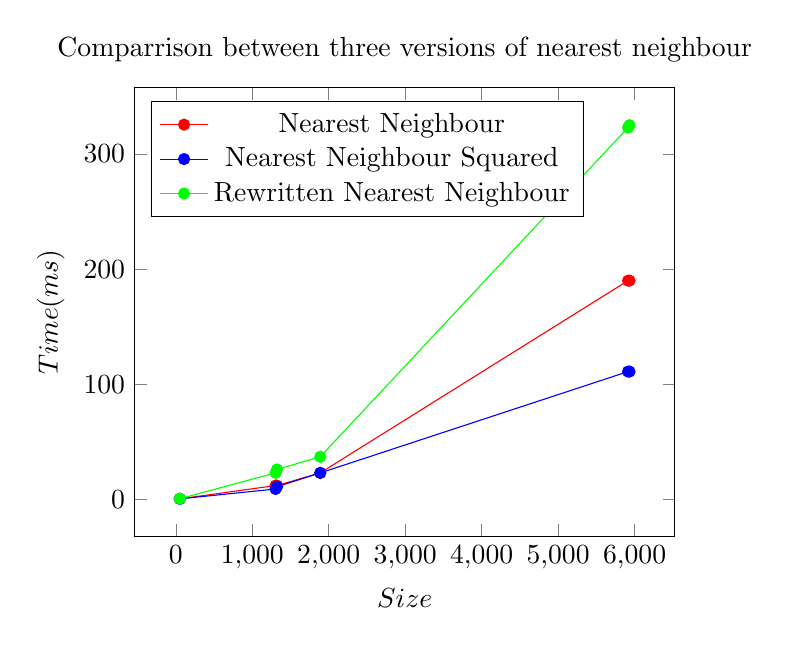
\begin{tikzpicture}
\begin{axis}[ 
title = Comparrison between three versions of nearest neighbour,
xlabel=$Size$,
ylabel={$Time (ms)$},
legend pos=north west
] 
\addplot [red,mark=*] coordinates {(52,0.45) (1304,12) (1323,12) (1889,23) (5915,190) (5934,190)};
\addplot [blue,mark=*] coordinates {(52,0.45) (1304,9) (1323,11) (1889,23) (5915,111) (5934,111)};
\addplot [green,mark=*] coordinates {(52,0.59) (1304,23) (1323,26) (1889,37) (5915,323) (5934,325)};
\addlegendentry{Nearest Neighbour}
\addlegendentry{Nearest Neighbour Squared}
\addlegendentry{Rewritten Nearest Neighbour}
\end{axis}
\end{tikzpicture}

Out of the three basic nearest neighbour algorithms the fastest algorithm is the one that leaves the distances to be compared against in their squared form as well as storing the value from the function as a variable instead of computing it twice. From the graph it is clear that there is a gain in performance from 2000 points onwards. Once there are 5934 points the improved algorithm has a 41.57\% improvement on computation time of the algorithm. The reason for this improvement is due to the distance function which does the following calculation:

\begin{equation}
Distance = \sqrt{x^2 + y^2}
\end{equation}
Where $x$ is (point A.x - point B.x) and $y$ is (point A.y - point B.y).

Therefore as the number of points increased the number of times this calculation also increased. As mathematical operations (especially square rooting) it clearly has a hit to performance like it is shown in the graph. Another reason for the nearest neighbour squared having quicker times is because the worst case scenario for the distance calculation has been reduced to one. In the original calculation the worst case scenario was two. This means that the number of times the operation is used is decreased significantly as the number of elements being sorted increases.

The rewritten nearest neighbour algorithm did not achieve the results that were aimed for. The reason for this is due to having more code executed in the for loop so as more iterations happened the longer it would take to compute the result. Even through the algorithm tried to reduce the number of iterations that happened the complexity of the algorithm still remained which means that regardless of hardware and software (for example development environment used) used it will always take longer than the default and the improved nearest neighbour algorithms.


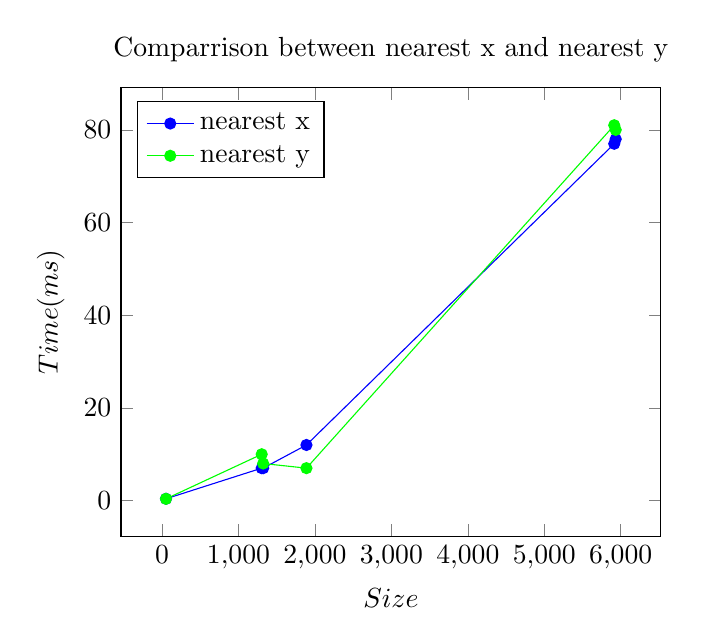
\begin{tikzpicture}
\begin{axis}[ 
title = Comparrison between nearest x and nearest y, 
xlabel=$Size$,
ylabel={$Time(ms)$},
legend pos=north west
] 
\addplot [blue,mark=*] coordinates {(52,0.39) (1304,7) (1323,7) (1889,12) (5915,77) (5934,78)};
\addplot [green,mark=*] coordinates {(52,0.38) (1304,10) (1323,8) (1889,7) (5915,81) (5934,80)};
\addlegendentry{nearest x}
\addlegendentry{nearest y}
\end{axis}
\end{tikzpicture}

In theory the nearest x and nearest y algorithms should have roughly the same time to compute the route due to the algorithms being the same apart from what axis it compares against. The nearest y also has an anomaly where the time taken briefly decreases for larger data sets. This may be due to background tasks stopping allowing more processing power to be dedicated to the algorithm. Apart from that the times are fairly consistent against each other. 



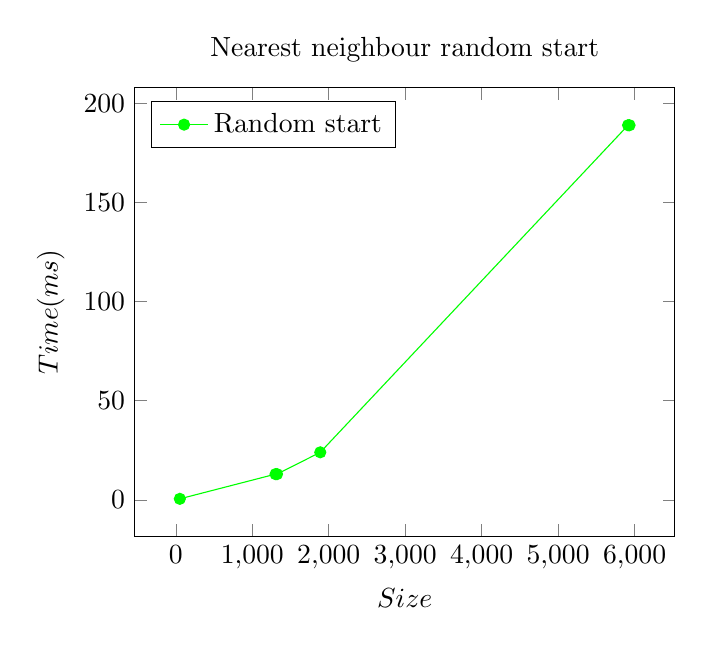
\begin{tikzpicture}
\begin{axis}[ 
title = Nearest neighbour random start, 
xlabel=$Size$,
ylabel={$Time(ms)$},
legend pos=north west
] 

\addplot [green,mark=*] coordinates {(52,0.53) (1304,13) (1323,13) (1889,24) (5915,189) (5934,189)};
\addlegendentry{Random start}
\end{axis}
\end{tikzpicture}

Random start has a similar trend in time compared to the original nearest neighbour algorithm. The reason the graph for the shuffle is not included in the results is because conceptually it does the same as the random start algorithm, mostly a little slower as it has a randomise a n size arrayList. 



The following graph shows the data size against the total distance the route provides. As the optimised and rewritten algorithms were only aiming to improve the time taken to calculate the nearest neighbour they will be omitted as the route is the exact same as the nearest neighbour and evidence of this is provided in the tables above. 


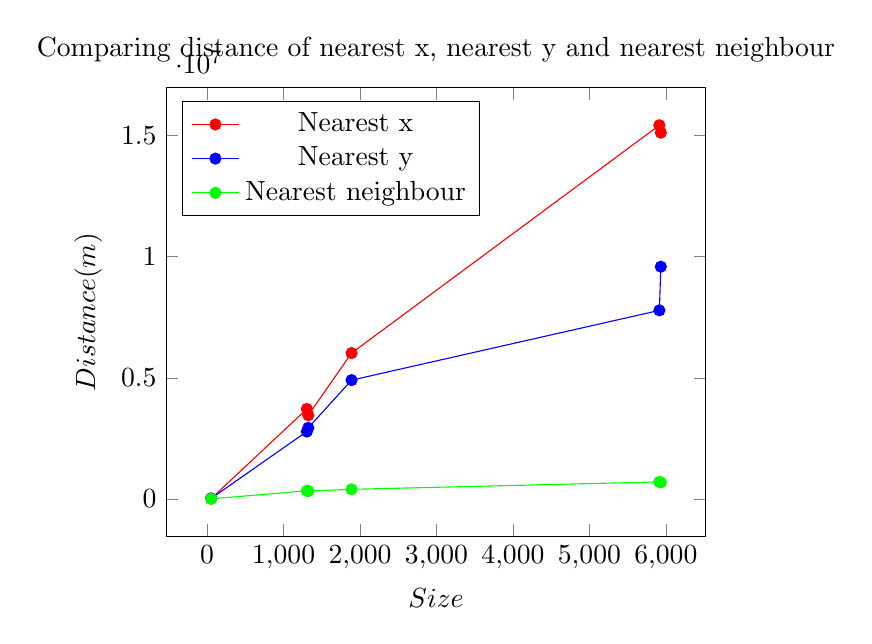
\begin{tikzpicture}
\begin{axis}[ 
title =  {Comparing distance of nearest x, nearest y and nearest neighbour},
xlabel=$Size$,
ylabel={$Distance (m)$},
legend pos=north west
] 
\addplot [red,mark=*] coordinates {(52,17074.13) (1304,3718084) (1323,3460174.47) (1889,6024698.02) (5915,15429176.67) (5934,15122594.14)};
\addplot [blue,mark=*] coordinates {(52,24438.27) (1304,2786850.75) (1323,2940280.95) (1889,4907965.14) (5915,7787705.43) (5934,9589407.52)};
\addplot [green,mark=*] coordinates {(52,8980.92) (1304,339797.47) (1323,332094.97) (1889,400684.64) (5915,707498.63) (5934,683805.99)};
\addlegendentry{Nearest x}
\addlegendentry{Nearest y}
\addlegendentry{Nearest neighbour}
\end{axis}
\end{tikzpicture}

As three of the variations were just the nearest neighbour (or attempts to improve it) the results were the same. Comparing the distances of nearest x and nearest y there is a clear improvement using the nearest y algorithm. Regardless of sample size the nearest neighbour always provided smaller distances. Therefore in situations where the distance is important this algorithm is more appropriate than the nearest x and y algorithms. 

From the results obtained an education assumption can be made about the nearest x and nearest y distances and that is the point distribution in the data set is what determines the total distance. For example a point distribution focused around a x-axis range of 0-5 but spread out far on the y-axis then the nearest axis would clearly return a smaller distance and vice-versa. However due to lack of control over what the point distribution would be these algorithms should not be recommended if a short distance is required. \paragraph{Route}\hfill

 The following section show the dataset rl5915 and the route calculated.
\onecolumn
\begin{figure}[h]
	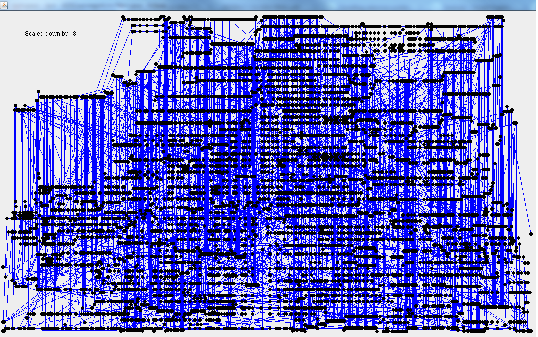
\includegraphics[width=\columnwidth]{images/rl5915unsorted.png}
	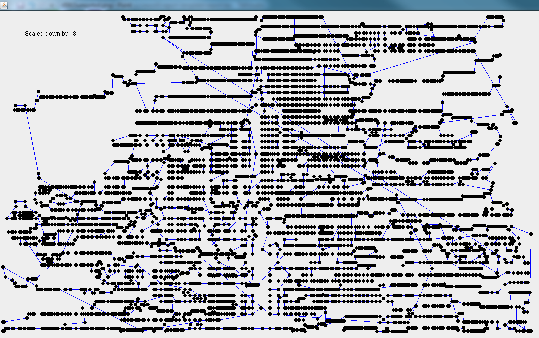
\includegraphics[width=\columnwidth]{images/rl5915nn.png}
	\caption{Unsorted route vs nearest neighbour.}
\end{figure}

\begin{figure}[h]
		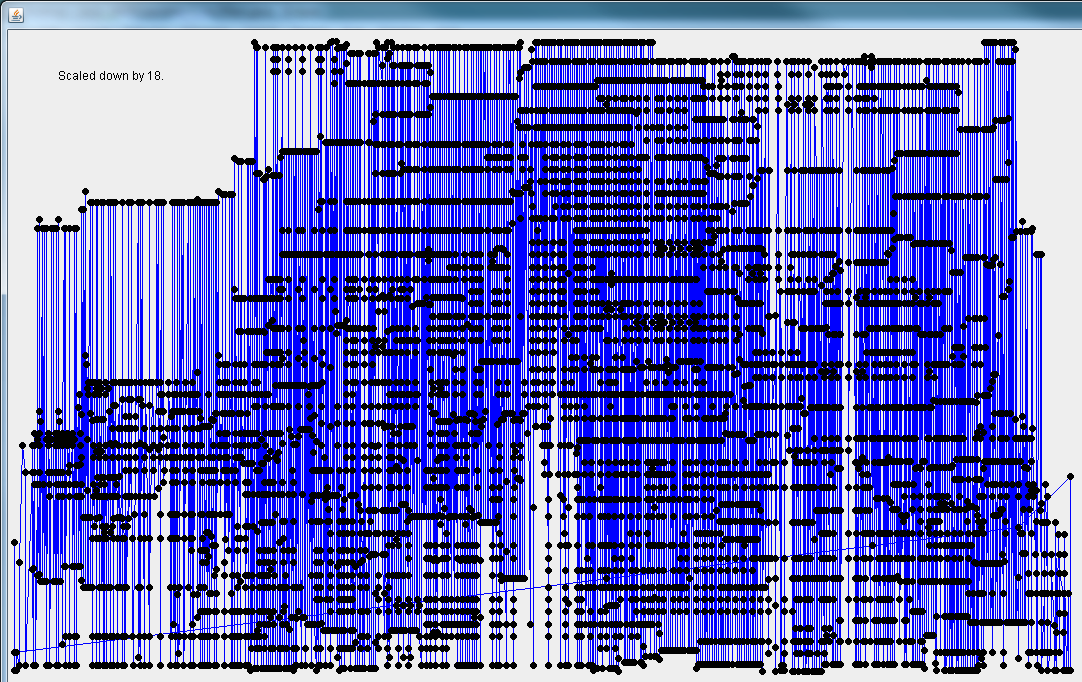
\includegraphics[width=\columnwidth]{images/rl5915nx.png}
			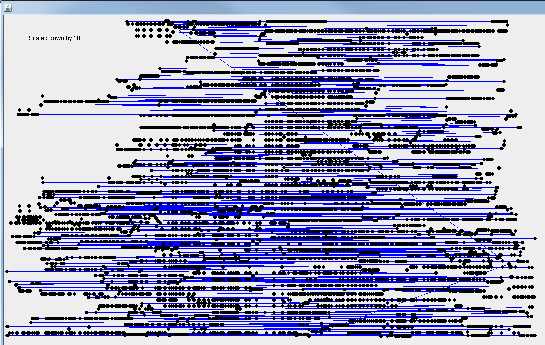
\includegraphics[width=\columnwidth]{images/rl5915ny.png}
	\caption{Nearest x vs nearest y.}
\end{figure}
\twocolumn
\section{Conclusion}

To conclude this report, with all the variations tested the best one overall was the nearest neighbour squared. This provides the same distance as the original nearest neighbour however the improvement in the time taken to compute the route has improved significantly. What is interesting to note is that even though the nearest x also had very fast computations majority of the time the route it returned was worse than just leaving the list unsorted. 

Possible improvement that can be made to the nearest neighbour algorithm that was implemented in this report is storing the result from the algorithm into an array instead of an arrayList. This would be possible as the size would be known as it would be the same as the input array. Also just using the input array to store the results instead of creating a copy of it in the algorithm would improve the computation time. This was not implemented as it would make checking the results to ensure that they are valid. Further research into '2-opt' could provide a good way of improving the results obtained from the nearest neighbour algorithm at the cost of a longer run time.

\section{Source code}
 The following source code provided should contain all the classes required to recreate the solution. If there are any errors (there should not be) please Email at 40167111@live.napier.ac.uk.
 
 To run the solution first type in the data set where it is loaded in (TsbLoader.loadTSPLib());
 Secondly chose what algorithm wants to be run by leaving it as the only uncommented algorithm. Having two algorithms will produce 
\onecolumn
\begin{verbatim}
import java.awt.geom.Point2D;
import java.util.ArrayList;
public class Main
{
	public static void main(String[] args)
	{
		Results result = new Results();		
		//File path to tsp's . 
		String data1 = "..//ADSCoursework//src//rl5915.tsp";
		String data2 = "..//ADSCoursework//src//rl1323.tsp";
		String data3 = "..//ADSCoursework//src//rl5934.tsp";
		String data4 = "..//ADSCoursework//src//rl1304.tsp";
		String data5 = "..//ADSCoursework//src//rl1889.tsp";
		String data6 = "..//ADSCoursework//src//berlin52.tsp";
		
		// Load data points into arraylist.
		ArrayList<Point2D> cities = new ArrayList<Point2D>(TsbLoader.loadTSPLib(data1));
		
		// Create arrayList for results to be stored in. Same size as in cities.
		// This should be slightly as size is already known.
		
		ArrayList<Point2D> results = new ArrayList<Point2D>(cities.size());
		// Loop is for repeatability. When recording results remove slowest and fastest extremes for me accuracy.
		//for(int i =0; i <5; i++)
		{
			// Start time when algorithm is about to run.
			long startTime = System.currentTimeMillis();
			
			// ---- Only run one method for algorithm below this or results are inaccurate! ---- \\
			
			// results = NearestNeighbourAlgorithm.NearestNeighbour(cities);
			// results = NearestNeighbourAlgorithm.NearestNeighbourRandStart(cities);
			// results = NearestNeighbourAlgorithm.NearestNeighbourShuffle(cities);
			// results = NearestNeighbourAlgorithm.NearestNeighbourSQ(cities);
			// results = NearestNeighbourAlgorithm.NearestNeighbourRewrite(cities);
			results = NearestNeighbourAlgorithm.NearestXNeighbour(cities);
			// results = NearestNeighbourAlgorithm.NearestYNeighbour(cities);
			
			// Stop time once algorithm is finished.
			long stopTime = System.currentTimeMillis();
			// Calculate how long it took.
			long elapsedTime = stopTime - startTime;
			// Add result to list of times.
			result.AddTimeToArray(elapsedTime);
			// ---- Timing is finished can check results now. ---- \\
			
		}
		
		/*	NOTE: because nearest neighbour will always return the same distance there is
		*  no purpose of storing multiple results. 
		*  When recording the results from Random start and Shuffle I stored and calculated the average by hand.
		*  TO DO: Store each of the results and automatically calculate average.
		*/
		
		// This will take the final result and store it.
		result.SetResults(results);
		
		// Print results.
		result.PrintResults(cities);	
	}
}

import java.awt.geom.Point2D;
import java.io.BufferedReader;
import java.io.FileReader;
import java.io.IOException;
import java.util.ArrayList;

public class TsbLoader
{
	TsbLoader(){}
	public static ArrayList<Point2D> loadTSPLib(String fName)
	{
		//Load in a TSPLib instance. This example assumes that the Edge weight type is %EUC_2D.
		//It will work for examples such as rl5915.tsp. Other files such as
		//fri26.tsp .To use a different format, you will have to
		//modify the this code
		ArrayList<Point2D> result = new ArrayList<Point2D>();
		BufferedReader br = null;
		try
		{
			String currentLine;
			int dimension =0;//Hold the dimension of the problem
			boolean readingNodes = false;
			br = new BufferedReader(new FileReader(fName));
			while ((currentLine = br.readLine()) != null)
			{
				//Read the file until the end;
				if (currentLine.contains("EOF"))
				{
					//EOF should be the last line
					readingNodes = false;
					//Finished reading nodes
					if (result.size() != dimension)
					{
						//Check to see if the expected number of cities have been loaded
						System.out.println("Error loading cities");
						System.exit(-1);
					}
				}
				if (readingNodes)
				{
					//If reading in the node data
					String[] tokens = currentLine.split(" ");
					//Split the line by spaces.
					//tokens[0] is the city id and not needed in this example
					float x = Float.parseFloat(tokens[1].trim());
					float y = Float.parseFloat(tokens[2].trim());
					//Use Java's built in Point2D type to hold a city
					Point2D city = new Point2D.Float(x,y);
					//Add this city into the arraylist
					//	System.out.println("Adding: " + city.toString());
					result.add(city);
				}
				if (currentLine.contains("DIMENSION"))
				{
					//Note the expected problem dimension (number of cities)
					String[] tokens = currentLine.split(":");
					dimension = Integer.parseInt(tokens[1].trim());
				}
				if (currentLine.contains("NODE_COORD_SECTION"))
				{
					//Node data follows this line
					readingNodes = true;
				}
			}
		}
		catch (IOException e)
		{
			e.printStackTrace();
		}
		finally
		{
			try
			{
				if (br != null)
				br.close();
			}
			catch (IOException ex)
			{
				ex.printStackTrace();
			}
		}
		return result;
	}	
}

import java.awt.geom.Point2D;
import java.util.ArrayList;
import java.util.HashSet;
import java.util.Set;

/* This utility class is here to provide helper methods*/
public class Util
{
	public static double routeLength(ArrayList<Point2D> cities)
	{
		//Calculate the length of a TSP route held in an ArrayList as a set of Points
		double result=0;//Holds the route length
		Point2D prev = cities.get(cities.size()-1);
		//Set the previous city to the last city in the ArrayList as we need
		// to measure the length of the entire loop
		for(Point2D city : cities)
		{
			//Go through each city in turn
			result += city.distance(prev);
			//get distance from the previous city
			prev = city;
			//current city will be the previous city next time
		}
		return result;
	}
	
	
	// This method is here to ensure that all cities are included.
	public static Boolean CheckLists(ArrayList<Point2D> original, ArrayList<Point2D> results)
	{
		// By turning the results into a set I can ensure that there are no duplicates by comparing to original size.
		Set<Point2D> set = new HashSet<Point2D>(results);
		if (set.size() != original.size())
		{
			System.out.println("Output size is not equal size to the input size.");
			return false;
		}
		else
		{
			// Create copies of original input and results to check.
			ArrayList<Point2D> o = new ArrayList<Point2D>(original);
			// Can use the instead of creating new arrayList to save memory/processing power.
			
			// Make sure each point in results are in original data set.
			for(Point2D r : original)
			{
				// point is in list. Remove to make search quicker
				if(o.contains(r) == false)
				{
					System.out.println("Results is missing: "+ r.toString());
					return false;
				}
				// r must be in list so remove it to speed comparison.
				o.remove(r);
			}
		}
		return true;
	}	
}

import java.awt.Color;
import java.awt.Dimension;
import java.awt.Graphics;
import java.awt.Polygon;
import java.awt.geom.Point2D;
import java.util.ArrayList;

import javax.swing.JFrame;
import javax.swing.JPanel;

/*This class is used to visually display the route calculated by the algorithm*/

public class DrawRoute extends JPanel
{
	private static final long serialVersionUID = 1L;
	private JFrame mainMap;
	private Polygon poly;
	
	public DrawRoute(){}
	
	public void Route(final ArrayList<Point2D> points)
	{
		// Visually approximate, but good enough.
		mainMap = new JFrame();
		mainMap.setResizable(true);
		
		mainMap.setDefaultCloseOperation(JFrame.DISPOSE_ON_CLOSE);
		
		int[] xCoords = new int[points.size()];
		int[] yCoords = new int[points.size()];
		for(int i =0; i < points.size();i++)
		{
			xCoords[i] = (int)points.get(i).getX()/18;
			yCoords[i] = (int)points.get(i).getY()/18;
		}
		poly = new Polygon(xCoords, yCoords, xCoords.length);
		JPanel p = new JPanel()
		{
			private static final long serialVersionUID = 1L;
			@Override
			protected void paintComponent(Graphics g)
			{
				super.paintComponent(g);
				g.setColor(Color.BLACK);
				
				g.drawString("Scaled down by 18.",50,50);
				g.setColor(Color.BLUE);
				g.drawPolygon(poly);
				g.setColor(Color.BLACK);
				for(int i=0; i < points.size();i++)
				{
					DrawNthPoint(g,poly,i);
				}
			}
			
			private void DrawNthPoint(Graphics g, Polygon polygon, int nth)
			{	        	
				int x = polygon.xpoints[nth];
				int y = polygon.ypoints[nth];
				g.drawOval(x-3,y-3,6,6);
				g.fillOval(x-3,y-3,6,6);
			}
			@Override
			public Dimension getPreferredSize()
			{
				return new Dimension(1980, 1080);
			}
		};
		mainMap.add(p);
		mainMap.pack();
		mainMap.setVisible(true);
	}
}
import java.awt.geom.Point2D;
import java.util.ArrayList;
import java.util.Collections;
import java.util.Random;


public class NearestNeighbourAlgorithm
{
	
	public static ArrayList<Point2D> NearestNeighbour(ArrayList<Point2D> inCities)
	{
		// This is the default nearest neighbour algorithm. The other methods are based on this. 
		
		ArrayList<Point2D> cities = new ArrayList<Point2D>(inCities);
		ArrayList<Point2D> result = new ArrayList<Point2D>();
		// Set current city.
		Point2D currentCity = cities.remove(0);
		
		// Closest city to the current city.
		Point2D closest = null;
		// While cities left in list.
		while (result.size() != inCities.size())
		{
			// Add current city to list.
			if(!result.contains(currentCity))
			result.add(currentCity);
			// Find closest city.
			double distance = Double.MAX_VALUE;
			for(Point2D t : cities)
			{
				if(Point2D.distance(currentCity.getX(), currentCity.getY(), t.getX(), t.getY()) < distance)
				{
					closest = t;
					distance = Point2D.distance(currentCity.getX(), currentCity.getY(), t.getX(), t.getY());
				}
				
			}
			cities.remove(closest);
			currentCity = closest;
			
		}
		return result;	
	}
	
	public static ArrayList<Point2D> NearestNeighbourSQ(ArrayList<Point2D> inCities)
	{
		
		// This is a more optimised version of the original algorithm.
		
		ArrayList<Point2D> cities = new ArrayList<Point2D>(inCities);
		ArrayList<Point2D> result = new ArrayList<Point2D>();
		// Set current city.
		Point2D currentCity = cities.remove(0);
		
		// Closest city to the current city.
		Point2D closest = null;
		// While cities left in list.
		while (result.size() != inCities.size())
		{
			// Add current city to list.
			if(!result.contains(currentCity))
			result.add(currentCity);
			// Find closest city.
			double distance = Double.MAX_VALUE;
			for(Point2D t : cities)
			{
				double dist = Point2D.distanceSq(currentCity.getX(), currentCity.getY(), t.getX(), t.getY());  
				if(dist < distance)
				{
					closest = t;
					distance = dist;
				}
				
			}
			cities.remove(closest);
			currentCity = closest;
			
		}
		return result;	
	}
	
	public static ArrayList<Point2D> NearestNeighbourRandStart(ArrayList<Point2D> inCities)
	{
		// This method just randomises the starting point. 
		Random rand = new Random();
		
		ArrayList<Point2D> cities = new ArrayList<Point2D>(inCities);
		ArrayList<Point2D> result = new ArrayList<Point2D>();
		// Set current city.
		Point2D currentCity = cities.get(rand.nextInt(cities.size()-1));
		
		// Closest city to the current city.
		Point2D closest = null;
		// While cities left in list.
		while (result.size() !=inCities.size())
		{
			// Add current city to list.
			if(!result.contains(currentCity))
			result.add(currentCity);
			// Find closest city.
			double distance = Double.MAX_VALUE;
			for(Point2D t : cities)
			{
				if(Point2D.distance(currentCity.getX(), currentCity.getY(), t.getX(), t.getY()) <= distance)
				{
					closest = t;
					distance = Point2D.distance(currentCity.getX(), currentCity.getY(), t.getX(), t.getY());
				}
			}
			cities.remove(closest);
			currentCity = closest;
		}
		return result;	
	}
	
	public static ArrayList<Point2D> NearestNeighbourShuffle(ArrayList<Point2D> inCities)
	{
		/* NOTE: THIS METHOD TECHNICALLY IS NO DIFFERENT FROM CHOOSING A RANDOM START*/
		/* This is due to the fact the list is always sorted by nearest neighbour. */
		// This method randomises the list. Results are unpredictable.
		ArrayList<Point2D> cities = new ArrayList<Point2D>(inCities);
		Collections.shuffle(cities);
		ArrayList<Point2D> result = new ArrayList<Point2D>();
		// Set current city.
		Point2D currentCity = cities.remove(0);
		
		// Closest city to the current city.
		Point2D closest = null;
		// While cities left in list.
		while (result.size() != inCities.size())
		{
			// Add current city to list.
			result.add(currentCity);
			// Find closest city.
			double distance = Double.MAX_VALUE;
			for(Point2D t : cities)
			{
				if(Point2D.distance(currentCity.getX(), currentCity.getY(), t.getX(), t.getY()) <= distance)
				{
					closest = t;
					distance = Point2D.distance(currentCity.getX(), currentCity.getY(), t.getX(), t.getY());
				}
			}
			cities.remove(closest);
			currentCity = closest;
		}
		return result;	
	}
	
	
	public static ArrayList<Point2D> NearestNeighbourRewrite(ArrayList<Point2D> inCities)
	{
		// This method is not efficient. In theory it is supposed to half the iterations of the for loop
		// at the cost of an additional check in 
		
		ArrayList<Point2D> cities = new ArrayList<Point2D>(inCities);
		ArrayList<Point2D> result = new ArrayList<Point2D>();
		// Set current city.
		Point2D currentCity = cities.get(0);
		cities.remove(currentCity);
		
		// Closest city to the current city.
		Point2D closest = null;
		// While cities left in list.
		while (result.size() != inCities.size())
		{
			// Add current city to list.
			if(!result.contains(currentCity))
			result.add(currentCity);
			// Find closest city.
			double distance = Double.MAX_VALUE;
			for(int i=0; i < cities.size(); i++)
			{
				Point2D t = cities.get(i);
				double dist = Point2D.distance(currentCity.getX(), currentCity.getY(), t.getX(), t.getY());
				// Check if the current city 
				if( dist < distance)
				{
					closest = t;
					distance = dist;
				}
				// If there is another city after it check if that is closer.
				if (i+1 < cities.size())
				{
					Point2D n = cities.get(i+1);
					dist = Point2D.distance(currentCity.getX(), currentCity.getY(), n.getX(), n.getY());
					if( dist < distance)
					{
						closest = n;
						distance = Point2D.distance(currentCity.getX(), currentCity.getY(), n.getX(), n.getY());
						i++;
					}
					
				}	
			}
			cities.remove(closest);
			currentCity = closest;
			
		}
		return result;	
	}
	
	public static ArrayList<Point2D> NearestXNeighbour(ArrayList<Point2D> inCities)
	{
		// This method just checks along the x-axis.
		ArrayList<Point2D> cities = new ArrayList<Point2D>(inCities);
		ArrayList<Point2D> result = new ArrayList<Point2D>();
		// Set current city.
		Point2D currentCity = cities.get(0);
		
		// Closest city to the current city.
		Point2D closest = null;
		// While cities left in list.
		while (result.size() != inCities.size())
		{
			// Add current city to list.
			if(!result.contains(currentCity))
			result.add(currentCity);
			// Find closest city.
			double closestX = Double.MAX_VALUE;
			for(Point2D t : cities)
			{
				if( t.getX() < closestX)
				{
					closest = t;
					closestX = closest.getX();
				}
			}
			cities.remove(closest);
			currentCity = closest;
		}
		return result;	
	}
	
	public static ArrayList<Point2D> NearestYNeighbour(ArrayList<Point2D> inCities)
	{
		// This method just checks along the y-axis.
		ArrayList<Point2D> cities = new ArrayList<Point2D>(inCities);
		ArrayList<Point2D> result = new ArrayList<Point2D>();
		// Set current city.
		Point2D currentCity = cities.get(0);
		
		// Closest city to the current city.
		Point2D closest = null;
		// While cities left in list.
		while (result.size() != inCities.size())
		{
			// Add current city to list.
			if(!result.contains(currentCity))
			result.add(currentCity);
			// Find closest city.
			double closestY = Double.MAX_VALUE;
			for(Point2D t : cities)
			{
				if( t.getY() <= closestY)
				{
					closest = t;
					closestY = closest.getY();
				}
			}
			cities.remove(closest);
			currentCity = closest;
		}
		return result;	
	}	
}

import java.awt.geom.Point2D;
import java.util.ArrayList;

// DIFFERENT KINDS OF AVERAGES? - CUT SHORTEST AND LONGEST TIMES?

public class Results
{
	// Store a list of all the times taken.
	private ArrayList<Long> times;
	private ArrayList<Point2D> resultList;
	Results()
	{
		times = new ArrayList<Long>();
		resultList = new ArrayList<Point2D>();
	}
	
	public Long CalculateAverageTime()
	{
		long average = 0;
		for(Long time : times)
		average+= time;
		average /=times.size();
		
		return average;
	}
	
	public Long CalculateShortestTime()
	{
		long quickest = Long.MAX_VALUE;
		for(long t : times)
		if (t < quickest)
		quickest = t;
		return quickest;
	}
	
	public Long CalculateLongestTime()
	{
		long slowest = 0;
		for(long t : times)
		if (t > slowest)
		slowest = t;
		return slowest;
	}
	
	public void AddTimeToArray(Long t)
	{
		times.add(t);
	}
	
	
	public ArrayList<Point2D> GetResults()
	{
		return resultList;
	}
	public void SetResults(ArrayList<Point2D> r)
	{
		resultList = r;
	}
	
	public void PrintResults(ArrayList<Point2D> original)
	{
		// Check if results are valid. If not display sizes of both lists.
		if (Util.CheckLists(original,resultList))
		{
			for(int i =0; i < times.size();i++)
			System.out.println("Time:" + times.get(i));
			System.out.println(CalculateAverageTime());
			
			
			double cityDist = Util.routeLength(original);
			double resultDist = Util.routeLength(resultList);
			System.out.println("Original size: " +original.size() + " | Result size: "+resultList.size());    
			
			System.out.println("Original length: " +cityDist + " | Result length: "+resultDist);    
			System.out.println("Time taken: "+ CalculateAverageTime() + " milliseconds.");
			DrawRoute route = new DrawRoute();
			route.Route(original);
			DrawRoute route1 = new DrawRoute();
			route1.Route(resultList);
		}
		else
		{	
			System.out.println("Input: "+ original.size() + " | Output: " + resultList.size());
		}
	}
}

\end{verbatim}
% \section*{Acknowledgements}
\bibliographystyle{acmsiggraph}
\bibliography{report}


\end{document}

